\chapter{Control of robots using variable gear-ratio actuators}
\label{sec:ControlAndPlanningOfRobotUsingVariableGearRatioActuators}


\section{Modeling}
\label{sec:model}


\section{Model-based control approach}
\label{sec:HierachicalControlApproach}


\subsection{Optimal Gear ratio along a trajectory}

\subsection{Trajectory following controllers}

\subsubsection{R* Computed Torque}
\label{sec:RobustTrajectoryFollowingController}

\subsubsection{R* Sliding Mode Controller}

\subsubsection{Heuristic approach to minimize gearshift}


\subsection{Trajectory planning}
\label{sec:SamplingBasedTrajectoryPlanner}


\section{Dynamic programming approach}
\label{sec:DynamicProgrammingAproach}



\begin{figure}[H]
	\centering
		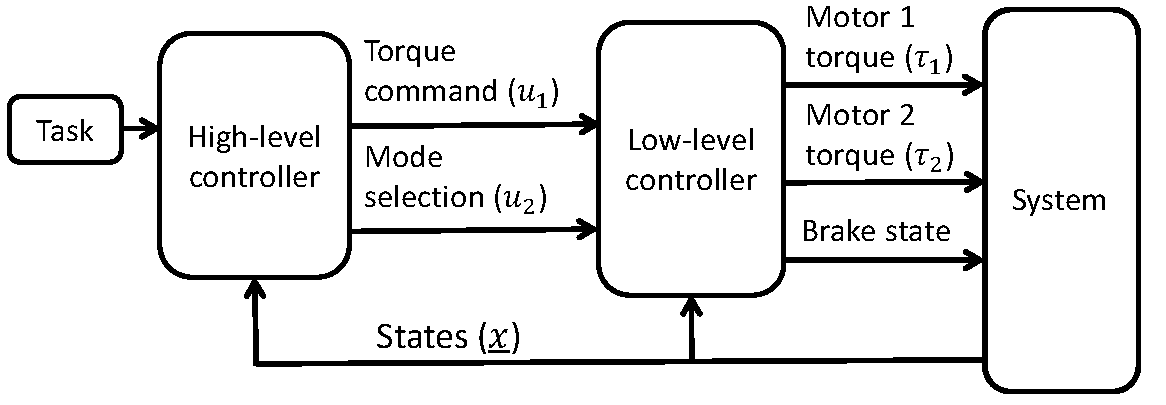
\includegraphics[width=0.45\textwidth]{blocks2.pdf}
	\caption{Controller architecture}
	\label{fig:blocks}
\end{figure}

\begin{figure}[H]
	\centering
		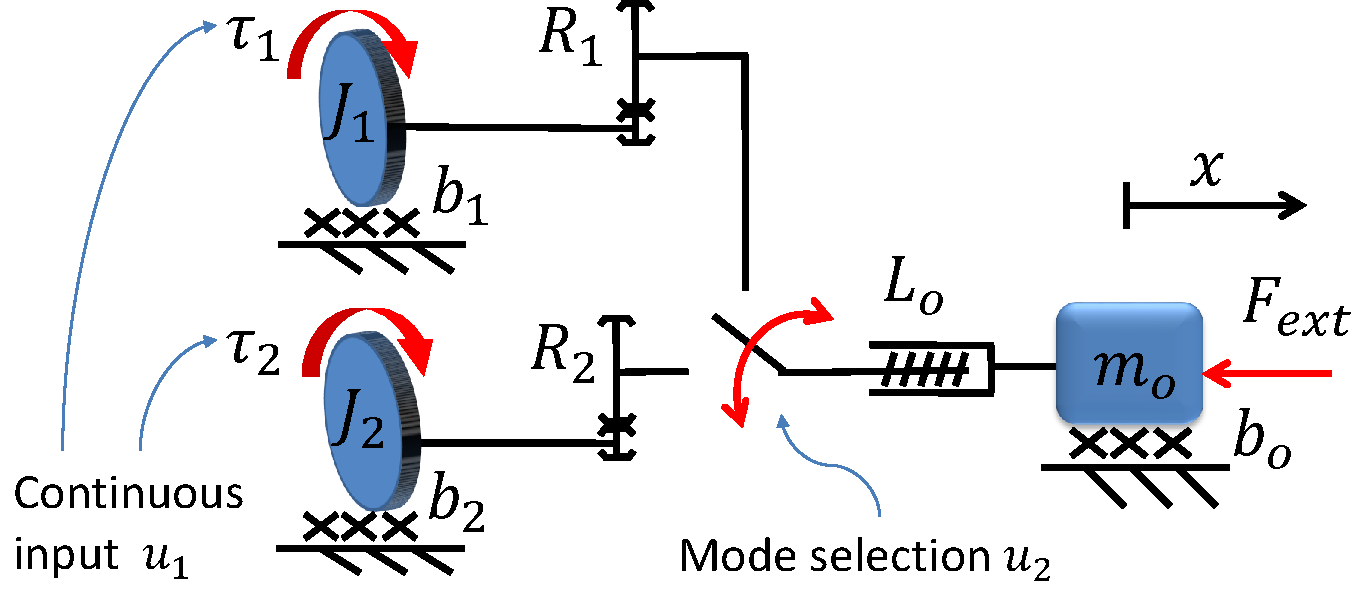
\includegraphics[width=0.42\textwidth]{model.pdf}
	\caption{Lumped parameter simplified model}
	\label{fig:model}
\end{figure}

\subsection{Value Iteration}


\begin{figure}[H]
        \centering
				\subfloat[Minimum time]{
        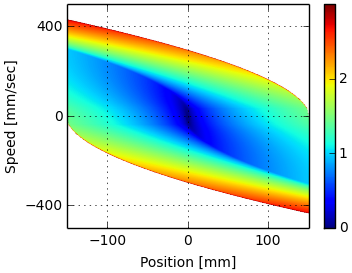
\includegraphics[width=0.32\textwidth]{Jt.png}
				\label{fig:J_time}}
        \subfloat[Quadratic cost]{
				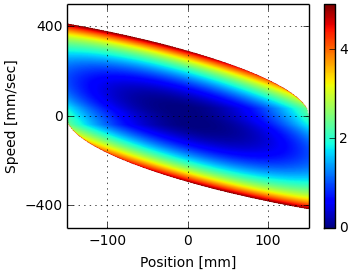
\includegraphics[width=0.32\textwidth]{Jq.png}%J_LQR.png
				\label{fig:J_LQR}}
				\subfloat[Minimum energy]{
				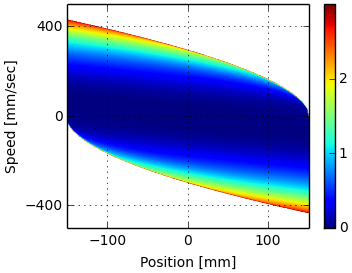
\includegraphics[width=0.32\textwidth]{Je.png}
				\label{fig:J_energy}}
        \caption{Optimal cost-to-go $J^*$}\label{fig:J}
\end{figure}

\begin{figure}[H]
        \centering
				\subfloat[Minimum time]{
        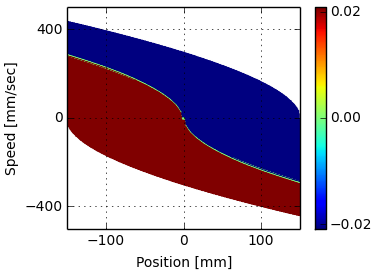
\includegraphics[width=0.32\textwidth]{u1t.png}
				\label{fig:u0_time}}
        \subfloat[Quadratic cost]{
				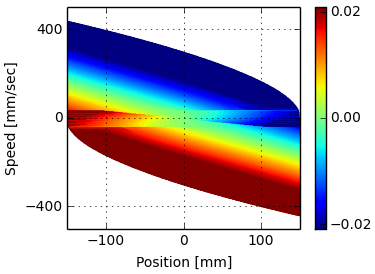
\includegraphics[width=0.32\textwidth]{u1q.png}
				\label{fig:u0_LQR}}
				\subfloat[Minimum energy]{
				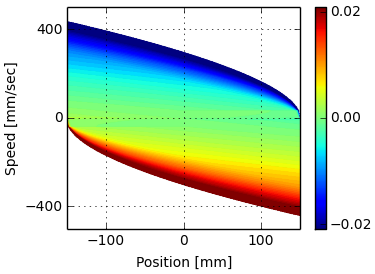
\includegraphics[width=0.32\textwidth]{u1e.png}
				\label{fig:u0_energy}}
        \caption{Optimal policy for the continuous torque command $u_1$ [Nm]}\label{fig:u0}
\end{figure}

\begin{figure}[H]
        \centering
				\subfloat[Minimum time]{
        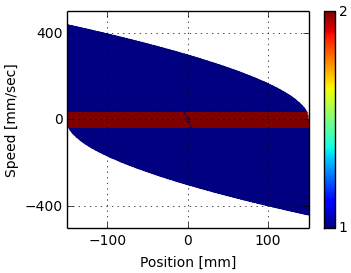
\includegraphics[width=0.32\textwidth]{u2t.png}
				\label{fig:u1_time}}
        \subfloat[Quadratic cost]{
				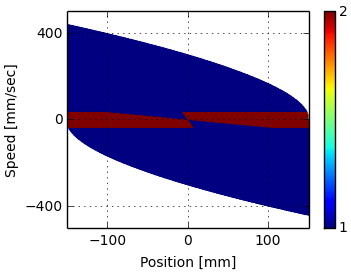
\includegraphics[width=0.32\textwidth]{u2q.png}
				\label{fig:u1_LQR}}
				\subfloat[Minimum energy]{
				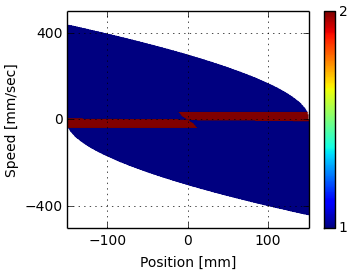
\includegraphics[width=0.32\textwidth]{u2e.png}
				\label{fig:u1_energy}}
        \caption{Optimal policy for the mode selection $u_2$}\label{fig:u1}
\end{figure}

\begin{figure}[H]
        \centering
				\subfloat[Minimum time]{
        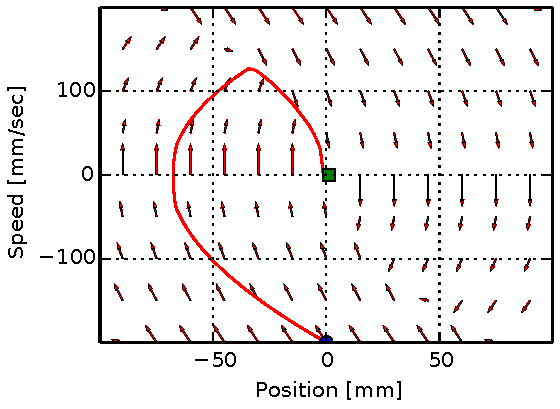
\includegraphics[width=0.32\textwidth]{ppt.pdf}
				\label{fig:phase_plane_time}}
        \subfloat[Quadratic cost]{
				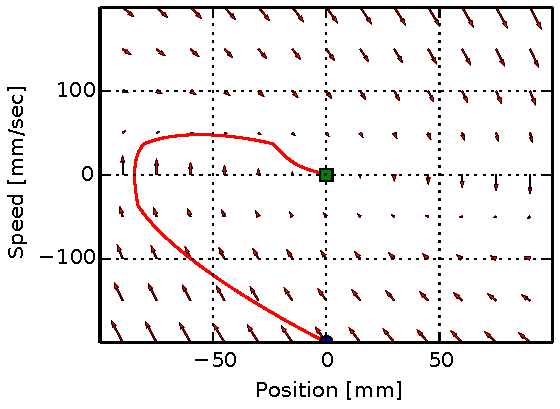
\includegraphics[width=0.32\textwidth]{ppq.pdf}
				\label{fig:phase_plane_LQR}}
				\subfloat[Minimum energy]{
				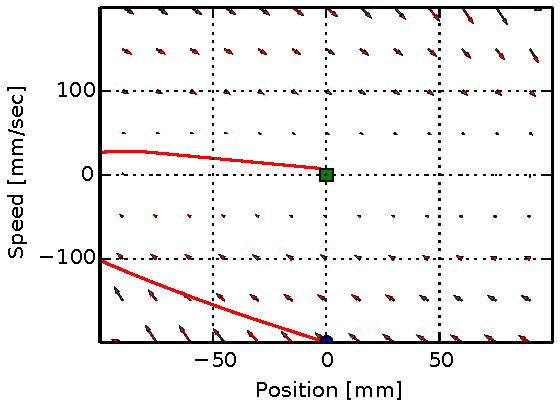
\includegraphics[width=0.32\textwidth]{ppe.pdf}
				\label{fig:phase_plane_energy}}
        \caption{Closed loop behavior with the optimal policy illustrated in the phase plane}\label{fig:phase_plane}
\end{figure}

\subsection{Reinforcement Learning}

